%%%%%%%%%%%%%%%%%%%%%%%
%%%%%%%%%%%%%%%%%%%%%%%
\begin{figure}[h!]
\begin{centering}
	\begin{subfigure}[b]{0.45\textwidth}	
		\centering
		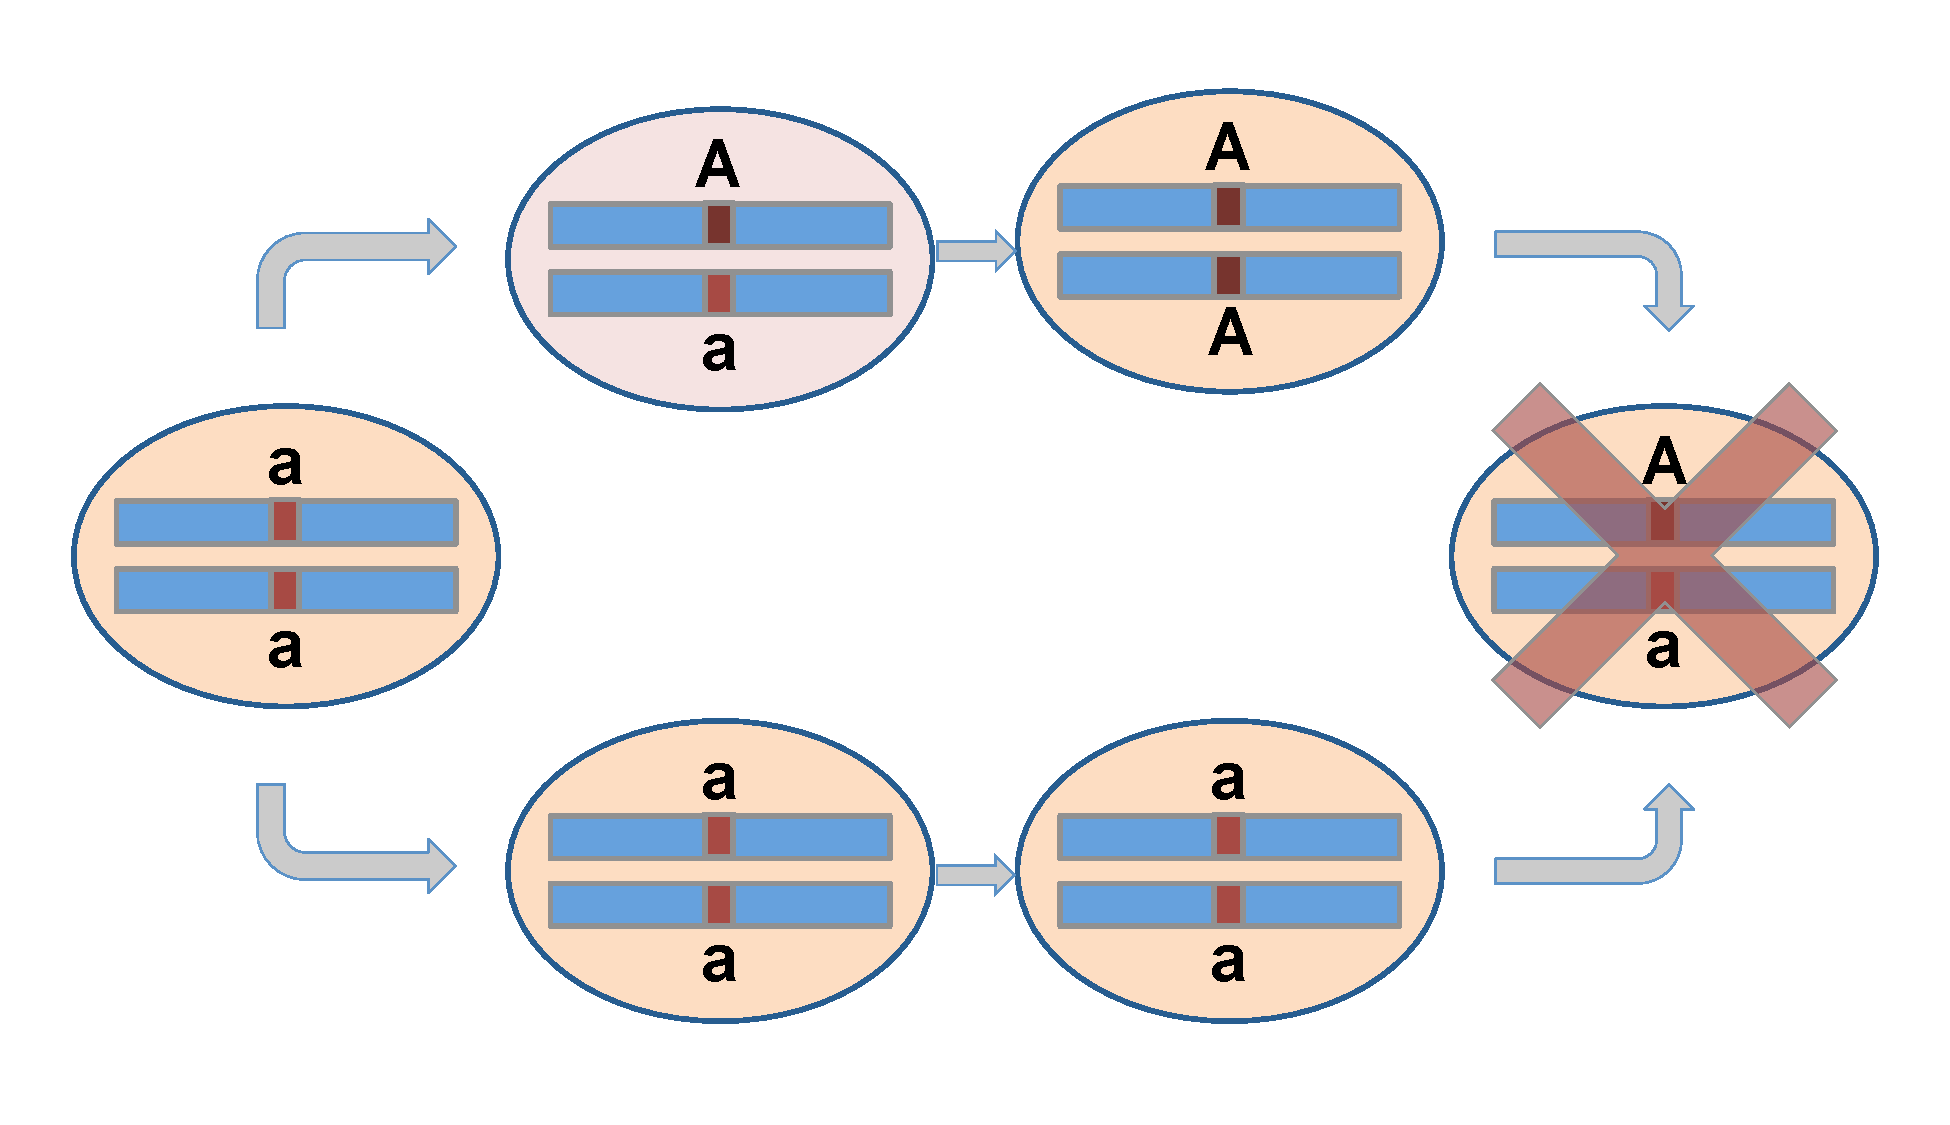
\includegraphics[width=\textwidth]{Figures/dm/DM_1}
		\label{fig:dm1}
		\caption{Single locus model of hybrid incompatibility}
	\end{subfigure}
	\quad
	\begin{subfigure}[b]{0.45\textwidth}	
		\centering
		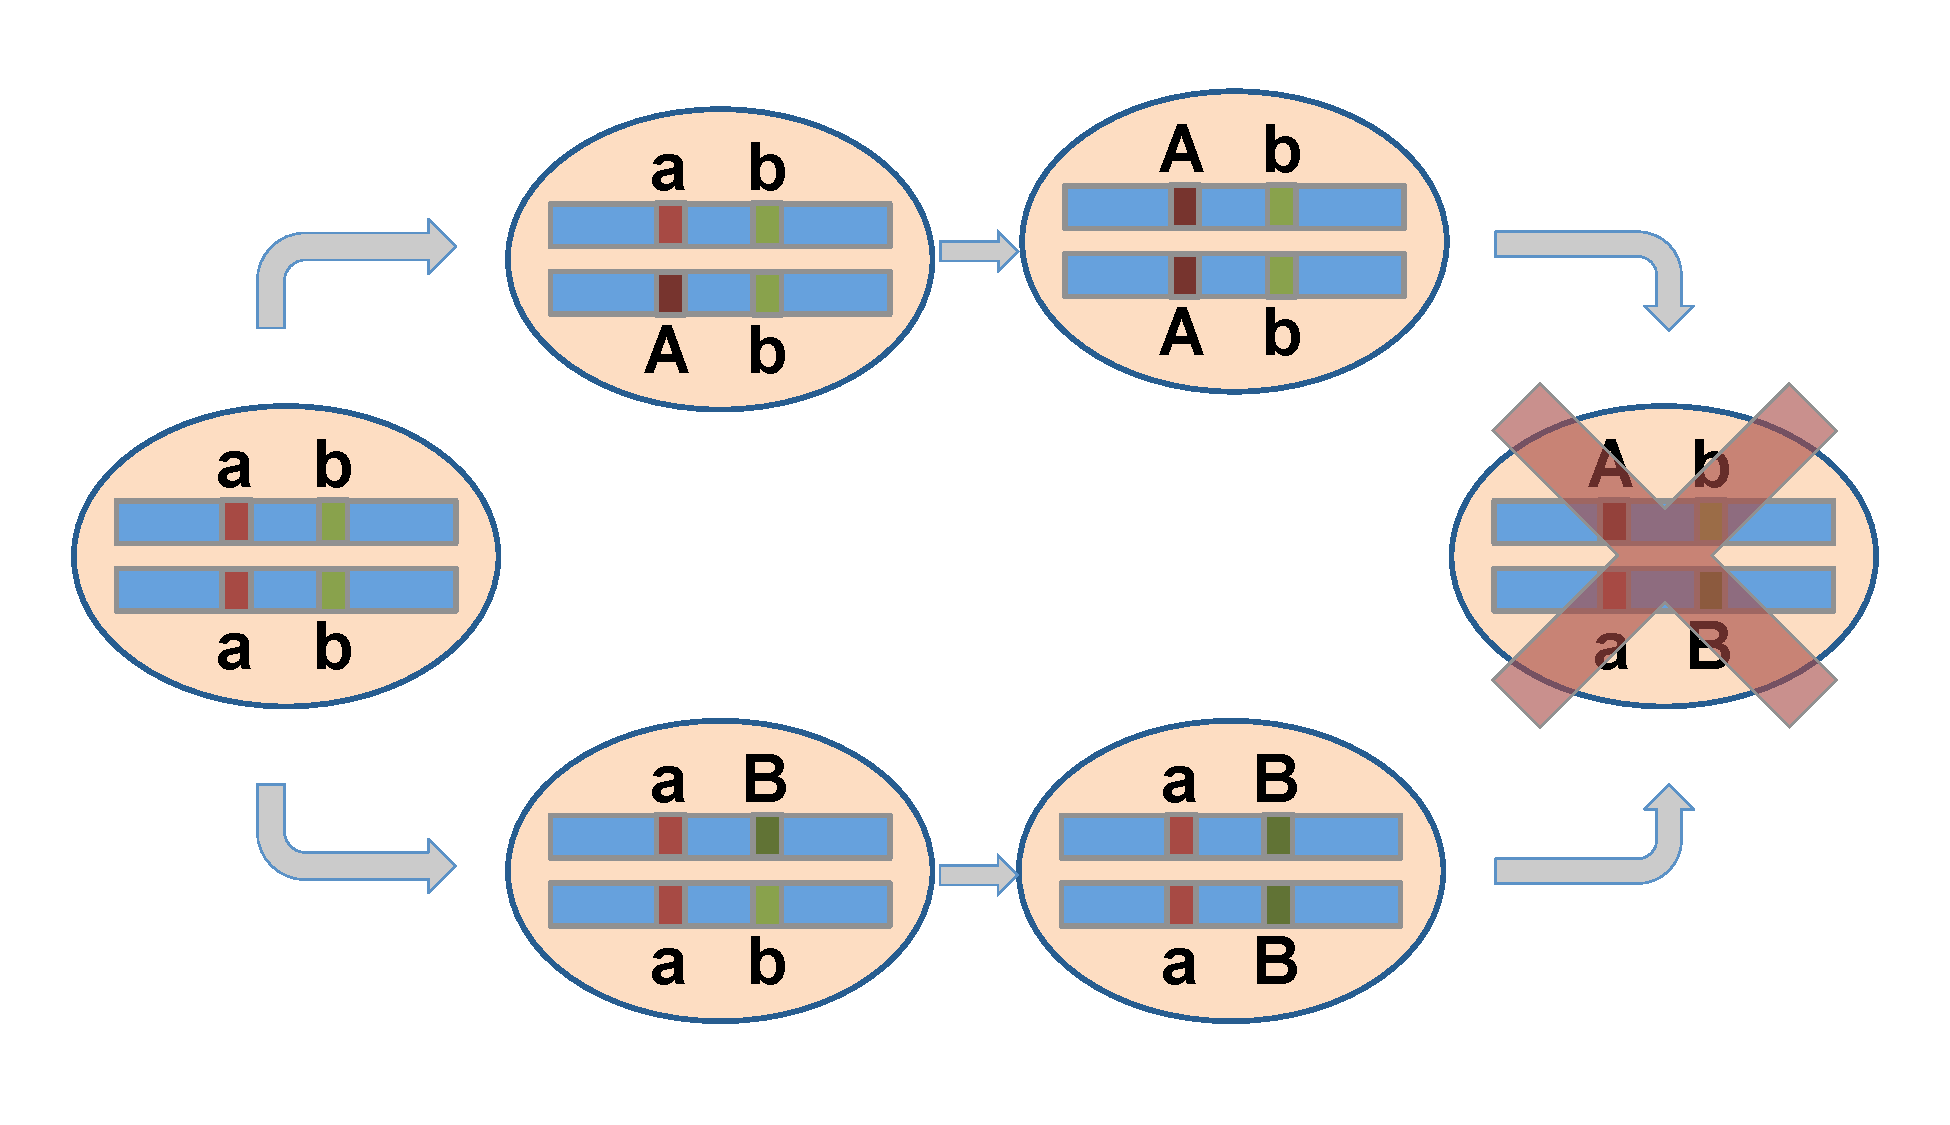
\includegraphics[width=\textwidth]{Figures/dm/DM_2}
		\label{fig:dm2}
		\caption{Two locus model of hybrid incompatibility}
	\end{subfigure}
\end{centering}
	
\caption[Description of the Dobzhansky-Muller model of hybrid incompatibilities]{A figure illustrating the concept behind the Dobzhansky-Muller model of hybrid incompatibilities.  \Cref{fig:dm1} illustrates a single locus model for hybrid incompatibility.  In this model only allele $a$ appears in the ancestral population. After becoming reproductively isolated the $A$ allele appears in one of the pure breeding populations and becomes fixed, but does not appear in the other.  Upon hybridization incompatibility is observed due to the $Aa$ combination of alleles, although this combination was previously experienced (light red organism) but did not result in incompatibilities. \Cref{fig:dm2} illustrates a multi-locus model for the development of hybrid incompatibilities.  In this model incompatibilities can be caused by incompatibilities between the $A$ and $B$ alleles, or by the $Aa$ combination of alleles occurring on the genetic background provided by the $B$ allele. Because the $A$ and $B$ only occurred on the same genetic background the two locus model avoids the problem of explaining how in the single locus model a genetic incompatibility can arise in an ancestral population without that population experiencing the same decrease in fitness as the hybrid species.}

\label{fig:dbm_simple}
\end{figure}
%%%%%%%%%%%%%%%%%%%%%%%
%%%%%%%%%%%%%%%%%%%%%%%
